\documentclass{article}
\usepackage[utf8]{inputenc}
\usepackage{enumerate}
\usepackage{tikz}
\usepackage{hyperref}
\usepackage{listings}
\usetikzlibrary{shapes.geometric, arrows}
\setlength{\tabcolsep}{18pt}
\usepackage{hyperref}
\usepackage{rotating}
\usepackage{multirow}
\usepackage{wrapfig}
\hypersetup{
    colorlinks = true,
    linkbordercolor = {white},
    linkcolor = {red},
}
\usepackage{geometry}
\geometry{
    a4paper,
    % total={170mm,257mm},
    left=16mm,
    right=16mm,
    top=10mm,
}

\title{Research Paper Review\\ WiLDNet: Design and Implementation of High Performance WiFi Based Long Distance Networks}
\author{Gohil Dwijesh \\ 2017CS50407}
\date{October 2019}

\begin{document}

\maketitle
\par This paper was written in 2007. The paper is mainly focused on WiFi-based Long Distance(WiLD) Networks. The author talks about the WiLD network, issues with existing approaches. He proposes the implementation and design of WiLDNet( WiFi-based Long Distance Network) to solve such issues. He experiments WiLDNet in his campus and Ghana and comes up with interesting conclusions that show the superiority of WiLDNet over existing approaches.
\par Developing countries and rural area require low-cost connectivity solutions. WiLD networks were emerging as low-cost connectivity solutions. Technologies used in the WiLD networks are low-cost low-power single board computers, high-volume low-cost off-the-shelf 802.11 wireless cards using an unlicensed spectrum. The author points out the following \textbf{issues} with such an approach: 802.11 protocol shortcomings that make it ill-suited for WiLD networks and links deployed in the WiLD network experienced high and variable loss rates due to external factors(mainly due to external WiFi interference).
\par The author proposes solutions for the aforementioned issues as described below.
\begin{enumerate}
    \item \textbf{802.11 protocol shortcomings}
    \begin{itemize}
        \item \textbf{Stop-And-Wait Protocol}
        \par \textbf{Issue:} The 802.11 MAC protocol uses a \textit{stop-and-wait} protocol. According to this protocol sender sends a packet, waits for its acknowledgment and then it can send the next packet. The sender can not send a new packet until it receives acknowledgment for the last sent packet. This \textit{stop-and-wait} protocol has two main drawbacks. First, under-utilization for long distance links. Second, unnecessary retransmissions due to acknowledgment time-out.
        \par \textbf{Solution:} To improve the link utilization, the author replaces the \textit{stop-and-wait} protocol with a sliding window-based flow control approach in which the receiver sends \textit{bulk acknowledgments} for a window of packets. The acknowledgment packets may contain data if required.
        \item \textbf{CSMA/CA}
        \par \textbf{Issue:} The 802.11 protocol uses CSMA/CA channel-access mechanism to avoid collisions. According to the mechanism sender node will listen to the medium for a fix duration of time and if it finds that there is no traffic in this duration then only it can send a packet. Over longer distance links, the sender may be unaware of traffic at the receiver due to propagation delay and this may result in collision at the receiver. As the propagation delay increases the probability of loss due to collision increases.
        \par \textbf{Solution:} The author proposes an implicit synchronization approach to solve this issue. Using \textit{Echo Protocol} and \textit{TDMA (Time Division Multiple Access)}, the sender and receiver can take turns to send and receive packets. From a node's perspective, time is divided into send and receive time slots.
        \item \textbf{Multiple Link Interference}
        \par \textbf{Issues:} The key idea is that high power radios create a strong RF field in the vicinity of the radio that can easily interfere with the transmission of the other radios on the same node having the same or overlapping channels. There are two types of problems that can arise. First, on the same node, let us say one radio starts transmitting then other radios will find the medium busy and will back off. Now in the WiLD network where there is a point to point communication with the independent receivers, such a back off results in suboptimal throughput. Second, transmission at the sender radio can interfere with the received signals at other radios on the same node.
        \par \textbf{Solution:} The author proposes \textit{Adaptive Loss Recovery} approach which is described later in this review. \textit{Adaptive Loss Recovery} is used to solve multiple link interference and external WiFi interference problem.
    \end{itemize}{}
    \item \textbf{Packet Losses due to External WiFi Interference}
    \par \textbf{Issue:} In case of WiLD network in urban mesh, \textit{Hidden Terminal Problem} becomes more pronounced. \textit{Hidden Terminal Problem} is when a sender node is not able to sense the traffic at the receiver due to propagation delay or longer distance links, and starts sending packets. This results in collisions at receiver.
    \par \textbf{Solution:} The author proposes an \textit{Adaptive Loss Recovery} approach using the \textbf{retransmissions} and \textbf{FEC} (Forward Error Correction). In FEC, the sender sends \textit{K} original packets and \textit{N-K} redundant packets. Redundancy factor is defined as \textit{N-K}/\textit{K}. FEC allows the receiver to correct the error packets up to an extent corresponding to redundancy factor without needing any retransmissions. There are two types errors observed due to external interference: CRC(Cyclic Redundancy Check) error and preamble error in which packets having preamble error results in packet drop. Intra-packet FEC helps recover packets with CRC error and inter-packet FEC to recover packets with preamble error. Therefore the author used an inter-packet FEC recovery system in WiLDNet implementation. Both approaches have trade-offs. Firstly, the loss rate can be reduced to zero if we arbitrarily increase the number of retransmissions but at the expense of increased delay. Secondly, increasing the redundancy factor reduces the loss rate at the extent of higher forward channel bandwidth or lowering the throughput. As the redundancy factor increases, the redundant data sent increases and throughput decreases.
\end{enumerate}{}
\begin{wrapfigure}{r}{0.5\textwidth}
    \begin{center}
        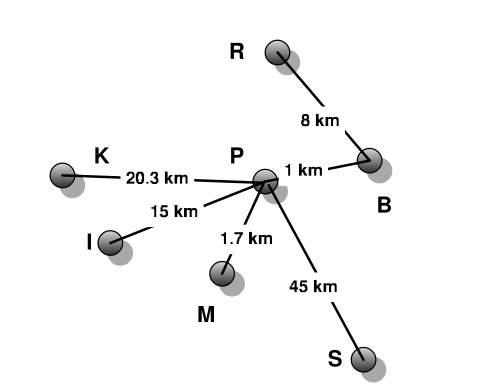
\includegraphics[width=0.48\textwidth]{campus_w.png}
    \end{center}{}
    \caption{Overview of WiLD campus testbed}
\end{wrapfigure}
\par The author uses three different experimental setups to conduct measurements and evaluate WiLDNet: Campus testbed, wireless channel emulator, and indoor multi-hop testbed. Figure 1 is real-world \textbf{campus testbed} on which the author deployed the WiLDNet. The campus testbed consists of links ranging from 1 to 45 km. The campus location has a variable level of external WiFi interference. \textbf{Wireless Channel Emulator} for repeatable experiments by keeping the link condition stable for the duration of the experiment and to emulate long links to study the effect of long propagation delay. The author performs controlled multi-hop experiments on an \textbf{Indoor Multi-hop Testbed} consisting of 4 nodes placed in RF isolated boxes. The setup was designed to recreate conditions similar to long outdoor links where transmissions from local radio interfere with each other. the extent of external interference can be configured using an additional node in each isolated box. This setup is used by the author to experiment and evaluate TDMA scheduling and loss recovery from interference.
\par The author draws some observations and conclusions that shows superiority of WiLDNet over existing approaches. 
\begin{itemize}
    \item \textbf{Stop-and-wait protocol:} Over long-distance links \textit{bulk acknowledgments} protocol is found to be 2-5 times better in cumulative throughput for TCP flows in both directions than stop-and-wait protocol.
    \item \textbf{Inter-Link Interference: } After implementing TDMA synchronization, WiLDNet yields 2.5x improvement in TCP throughput on real-world multi-hop setup.
\end{itemize}{}
\par The paper is oriented towards providing low-cost connectivity in developing countries and rural areas. The following are the recent works that explore a similar issue.
\begin{itemize}
    \item \textit{Soft-TDMAC: A Software TDMA-Based MAC over Commodity 802.11 Hardware:} They designed and implemented a soft-TDMAC, a software \textit{Time Division Multiple Access} based MAC protocol, running over commodity 802.11 hardware. Soft-TDMAC is capable of synchronizing all pairs of network clocks to within microseconds of each other.
    \item \textit{DTLSR: Delay Tolerant Routing for Developing Regions:}  By making small, yet critical, modifications to classical link-state routing, they demonstrated that their system operates effectively when conventional routing and forwarding may fail.
    \item \textit{Beyond Pilots: Keeping Rural Wireless Networks Alive:} The author presents low-cost and sustainable solutions for several aspects of the system including monitoring, power, backchannels, recovery mechanism and software. Deployment of such solutions leads to the scaling of two rural wireless networks.
\end{itemize}{}
\par There are some indirect assumptions taken by the author that can affect the applicability of the claims.
\begin{itemize}
    \item \textbf{Throughput Improvement} The improvement due to \textit{bulk acknowledgments} is more pronounced(4-5x) for links having a length greater than 100 km. There is no significant improvement due to \textit{bulk acknowledgments} compared to \textit{stop-and-wait protocol} for links with length smaller than 50 km. Where in the real world we can have links with smaller length.
    \item \textbf{TDMA scheduling:} In multi-hop experiment set-up the author uses 4 nodes kept in RF isolation box. This multi-hop set-up is used by the author to evaluate TDMA scheduling and loss recovery approach. In Real life, the number of hops/nodes can be larger. So larger number of hops may affect the TDMA scheduling delay.
\end{itemize}{}
\par Repeating these experiments can help exploit the weaknesses of current 802.11 policies giving a chance to make the system more robust. To carry out the experiment in current date, we need to better approximate our experimental set-up to real-world networks. We will need to use more hops and higher extent of external interference. From the studies the author did in 2007, he found that contribution of multipath interference to be negligible in packet losses. We may have to conduct the study again because that contribution may not be negligible in the current date.
\end{document}
